\documentclass[12pt,a4paper]{article}
\usepackage[utf8]{inputenc}
\usepackage{amsmath}
\usepackage{amsthm}
\usepackage{amsfonts}
\usepackage{amssymb}
\usepackage{tikz}
\usepackage{cancel}
\usetikzlibrary{arrows}
\newtheorem{theorem}{Theorem}
\newtheorem{definition}{Definition}
\usepackage[ruled,vlined]{algorithm2e}
\usepackage{verbatim}

\usepackage{mathtools}

\DeclarePairedDelimiterX{\klx}[2]{(}{)}{%
	#1\;\delimsize\|\;#2%
}
%\newcommand{\kl}{\mathrm{KL}\klx}
\newcommand{\kl}{D\klx}
\DeclarePairedDelimiter{\norm}{\lVert}{\rVert}

\begin{document}
\bibliographystyle{plain}
\title{Bayesian Inference}
\author{Viktor}
\maketitle

%\section{Graph theory}
\subsection{Basic definitions}
\begin{itemize}
\item definitions
\item triangulation
\end{itemize}
\subsection{Probabilistic graphs}
\paragraph*{Directed acyclic graphs}
\begin{itemize}
\item interpretation
\item not unique (bayes thm)
\item plate notation
\item model building
\item conditional independence
\end{itemize}
\paragraph*{Markov Networks}
\begin{itemize}
\item interpretation
\item conditional independence
\item Moralization
\end{itemize}
\subsection{Inference on Probabilistic graphs}
\paragraph*{Junction tree}
\paragraph*{•}
%\section{Probabilistc graphical models}
In principle there are three kind of graphical representations
directed acyclic graphs (DAG), markov networks, factor graphs
with addtional types of graphs, which emerge technically  upon inference  (such as clique graphs and junction trees).

\section{DAGs, Markov Networks and Factor Graphs}

\section{Training}
\section{Inference}
Inference is the process of 
%\section{Basics}
\begin{itemize}
\item Formal definition of a random variable
\item independence and conditional independence
\end{itemize}
Event $x$ and $y$ are  \textit{independent }$:\Leftrightarrow$ their joint distribution  factorizes $p(x,y)=p(x)p(y)$
The probability of an event $x$ conditioned on knowing event $y$  is called \textit{conditional probability}, $p(x|y) :=  \frac{p(x,y)}{p(y)}$
We also say the probability of $x$ given $y$. If $p(x)=0$ then $p(x|y)$ is not defined.
From this together with $p(x,y) = p(y,x)$ follows Bayes' rule.
\begin{theorem}[Bayes' rule]
\begin{align}
p(x|y) :=  \frac{p(y|x) p (x)}{p(y)}
\end{align}
\end{theorem} 
\paragraph{Indepenent and identically distributed.} This is a very common assumption. It is closely related to the notion of symmetry and exchangeable random variables, which eventually leads to the heart of statistical problems: how to characterize joint probabilities. This is turn is closely related to De Fetti's theorem \cite{barber}. However, for the time beeing we simple state its practical implication. Consider a variable $x$ and $n$ observations $x_1 \dots x_n$ of that variable. They are called  independent and identically distributed (IID) $:\Leftrightarrow$ if their joint probability factorizes.
\begin{align}
p(x_1, \dots, x_n) = \prod _ {i = 1} ^ n p(x_i)
\end{align}
Independent refers to the factorization is just the definition above. Identical means that each observation is drawn from the same underlying distribution.  

\paragraph*{Bayes' Inference.} The basic idea is to use Bayes' rule to obtain a distribution over the underlying model parameters of a random process. Let there be given a probability distribution $p(x|\theta)$, which is parametrized by $\theta \in \Theta$ with some parameter space $\Theta$ \footnote{Here we are inconsistent in our notation, because capitals usually is reserved for random variables, whereas here it is some parameter space}. For a set of $n$ observed data points $X=\{x_1,\dots, x_n\}$ Bayes' rule then reads:
\begin{align} \label{bayes_inference}
p(\theta|X) = \frac{p(X|\theta)p(\theta)}{p(X)}
\end{align}
The term $p(\theta|X)$ is called posterior distribution.

\paragraph*{Likelihood}
The term $p(X|\theta)$  in  (\ref{bayes_inference}) is called likelihood. It describes the probability of the data given the model, which is determined by the (fixed) model parameters $\theta$. How the likelihood is chosen is determined by the underlying random process. A common simplification is to assume IID observations, $p(X|\theta) = p(x_1, \dots, x_n|\theta) =   \prod _i  p(x_i | \theta)$. 

Sometimes it is convenient to work with the logarithm of the likelihood (log-likelihood). In the case of IID observations we get $\sum _i \log p(x_i | \theta)$. The log-likelihood is used if one tries to optimise the likelihood rather than the posterior with respect to $\theta$. Since the log is a strictly monotonic function the optimum remains invariant \footnote{consider a strictly monotonic, differentiable function g and a differentiable function g. Then $(g \circ f) '  = g'\circ f \cdot f'$. Since g is strictly monotonic $g' >0 $. Therefore the maximum of  $g \circ f$ is given by the maximum of $f$.}. The advantage is now that solving for $\theta$ is often easier for the log-likelihood than for the likelihood. 

\paragraph*{Maximum likelihood.} Instead of working with the full expression \ref{bayes_inference} when inferring $\theta$ one often works directly with the likelihood,
\begin{align}
\hat \theta = \text{arg sup}_\theta p(X|\theta).
\end{align}
This is eventually an manifestation of the likelihood principle \cite{robert}. Beside the advantages (eg, parametrization invariance, asympotitic properties) the maximum likelihood also has several drawbacks: in high dimensions it can be computationally complex to find the maximum or there could be more local maxima. Furthermore, there is no decision-theoretic and probabilistic support for this approach. In particular,  the map $\theta \mapsto p(X|\theta)$ is not a PDF over $\theta$ (whereas it is one for $p(\theta|X)$). This is a general property of conditional probabilities.\footnote{Consider 
a joint distribution $p(x, \theta)$ with constant marginals, $p(x) = \int p(x,\theta)\, d \theta =1/k$ on the interval $x = [0,k]$ and  $p(\theta) = \int p(x,\theta)\, d \theta =1/c$  on the interval $\theta = [0,c]$ with $k\neq c$.  Assume that the map $\theta \mapsto p(x|\theta)$ is a PDF. Then, $\forall x$  $1=\int_0^c p(x|\theta) \, d \theta = \int_0^c\frac{p(x,\theta)}{p(\theta)}\, d\theta =  c \int_0^cp(x,\theta)\, d\theta = c p(x) = \frac{c}{k} \neq 1$.}


%\section{Priors}
\paragraph*{Prior.} The term $p(\theta)$ is called prior distribution. It describes the uncertainty about the model parameter $\theta$ before observing (additional) data. So, it reflects our level of ignorance. Determining the prior is the most vodoo-part in the Bayesian approach. Infact it is the main point of criticism. Often one uses uninformative priors, (which are not necessarily uniform priors) or/and priors that are conjugate to a given likelihood function.
More details may be found in Ref. \cite{robert}, Chap. 3.
\subsection{Conjugate priors}
\begin{definition}[Conjugacy\cite{robert}] A family of $\mathcal F$ of probability distributions on $\Theta$ is called conjugate to a likelihood function $f(x|\theta) :\Leftrightarrow$  $\forall \pi \in \mathcal F$ the posterior distribution $\pi(\theta|x) \in \mathcal F$.  
\end{definition}
It is known that for the exponential family there always exists a conjugate prior. Furthermore conjugate priors are quite well studied.
Let's summarize the relevant ones for us in Table \ref{tab:conjugate_priors}.
\begin{table}
\begin{tabular}{lll}
\hline \hline
Likelihood & Prior &Posterior \\
$pk(x|\theta)$ & $\pi(\theta)$ & $\pi(\theta|x)$ \\
\hline
$ Bin (n, \theta)$ &  $Beta (\alpha, \beta)$ &  $Beta (\alpha +x, \beta + n -x)$  \\
$Mult_k(\theta_1 \dots \theta_k, n)$ 
& $Dir_k(\alpha_1 \dots \alpha_k)$   
& $Dir_k(\alpha_1 + x_1 \dots \alpha_k + x_k)$  \\
\hline\hline
\end{tabular}
\caption{\label{tab:conjugate_priors}Conjugate priors for given likelihoods.}
\end{table}
\paragraph*{Example: Conjugate Prior for the Binomial distribution.} This example shows that the Beta distribution is the conjugate prior to the binomial distribution. Assume the model for the data is $P(X|\theta)=Bin(x|\theta, n)$ ($\theta$ is the success probability and $n$ is the number of trials) and chose the Beta distribution as Prior, $P(\theta) = Beta(\theta|\alpha, \beta) $. Then we get as posterior
\begin{align} \label{eq:beta_binom}
p(\theta |x, n, \alpha, \beta) &=\frac{1}{N} Bin(x|n,\theta) Beta(\theta|\alpha, \beta) \\
& = \frac{1}{N}  \frac{\binom {n} {x} \theta^{x + \alpha-1} (1-\theta)^{n-x+\beta -1}}{B(\alpha, \beta)}  \\
& = Beta(\theta | x + \alpha, n-x+\beta),
\end{align} 
again a Beta distribution with updated parameters. The factor $1/N$ is just the normalization constant, which may be obtained be integrating the right hand side over $\theta$. The normalization requirement leads to the general trick to only consider the functional form of the free variables (in this case $\theta$) and identify the posterior distribution only via the functional form. The rest is done by the normalization requirement. For this example we would have
\begin{align}
 p(\theta |x, n, \alpha, \beta) &\propto Bin(x|n,\theta) Beta(\theta|\alpha, \beta) \\ 
 &\propto \theta^{x + \alpha-1} (1-\theta)^{n-x+\beta -1} \\ 
 &\propto Beta(\theta | x + \alpha, n-x+\beta)
\end{align}

In order to clarify how the conditionals in the first line emerge it's instructive to look at the joint distribution,
\begin{align*}
p(\theta, \alpha, \beta, n, x) = p(x|\theta, n) p(\theta|\alpha, \beta) p(n) p(\alpha) p(\beta)
\end{align*}
\begin{figure}
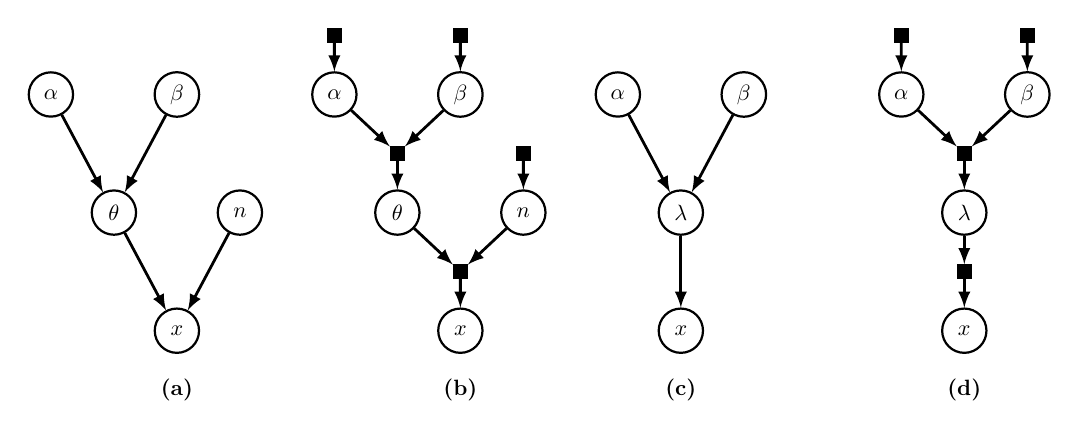
\begin{tikzpicture}[thick,xscale=0.8, yscale=.75, every node/.style={scale=0.8}]
\tikzset{vertex/.style = {shape=circle,draw,minimum size=2em}}
\tikzset{edge/.style = {->,> = latex, line width=1}}

% binomial beta directed graph
\begin{scope}
% vertices
\node[vertex] (a) at  (-1,2) {$\alpha$};
\node[vertex] (b) at  (1,2) {$\beta$};
\node[vertex] (x) at  (1, -2) {$x$};
\node[vertex] (n) at (2,0) {$n$};
\node[vertex] (t) at (0,0) {$\theta$};
%edges
\draw[edge] (a) to (t);
\draw[edge] (b) to (t);
\draw[edge] (t) to (x);
\draw[edge] (n) to (x);
\node at (1, -3) {\textbf{(a)}}; 
\end{scope}

% binomial beta factor graph
\begin{scope}[shift={(4.5,0)}]
% vertices
\node[vertex] (a) at  (-1,2) {$\alpha$};
\node[vertex] (b) at  (1,2) {$\beta$};
\node[vertex] (x) at  (1, -2) {$x$};
\node[vertex] (n) at (2,0) {$n$};
\node[vertex] (t) at (0,0) {$\theta$};
\begin{scope}[vertex/.style = {shape=rectangle, draw,minimum size=.1em, inner sep=3pt, fill=black}]
\node[vertex] (fone) at  (-1,3) {};
\node[vertex] (ftwo) at  (1,3) {};
\node[vertex] (fthree) at (0,1) {};
\node[vertex] (ffour) at (1,-1) {};
\node[vertex] (ffife) at (2,1) {};
\end{scope}
%edges

\draw[edge] (fone) to (a);
\draw[edge] (ftwo) to (b);
\draw[edge] (a) to (fthree);
\draw[edge] (b) to (fthree);
\draw[edge] (fthree) to (t);
\draw[edge] (t) to (ffour);
\draw[edge] (n) to (ffour);
\draw[edge] (ffour) to (x);
\draw[edge] (ffife) to (n);
\node at (1, -3) {\textbf{(b)}}; 
\end{scope}

% poisson gamma directed graph
\begin{scope}[shift={(9,0)}]
% vertices
\node[vertex] (a) at  (-1,2) {$\alpha$};
\node[vertex] (b) at  (1,2) {$\beta$};
\node[vertex] (l) at (0,0) {$\lambda$};
\node[vertex] (x) at (0,-2) {$x$};
%edges
\draw[edge] (a) to (l);
\draw[edge] (b) to (l);
\draw[edge] (l) to (x);
\node at (0, -3) {\textbf{(c)}}; 
\end{scope}

% poisson gamma factor graph
\begin{scope}[shift={(13.5,0)}]
% vertices
\node[vertex] (a) at  (-1,2) {$\alpha$};
\node[vertex] (b) at  (1,2) {$\beta$};
\node[vertex] (l) at (0,0) {$\lambda$};
\node[vertex] (x) at (0,-2) {$x$};
\begin{scope}[vertex/.style = {shape=rectangle, draw,minimum size=.1em, inner sep=3pt, fill=black}]
\node[vertex] (f1) at  (-1,3) {};
\node[vertex] (f2) at  (1,3) {};
\node[vertex] (f3) at  (0,1) {};
\node[vertex] (f4) at  (0,-1) {};
\end{scope}
%edges
\draw[edge] (f1) to (a);
\draw[edge] (f2) to (b);
\draw[edge] (a) to (f3);
\draw[edge] (b) to (f3);
\draw[edge] (f3) to (l);
\draw[edge] (l) to (f4);
\draw[edge] (f4) to (x);
\node at (0, -3) {\textbf{(d)}}; 
\end{scope}

\end{tikzpicture}


\caption{\label{fig:graphs_for_conj_priors}Directed graph (a) and factor graph (b) for beta distribution as conjugate prior of the binomial distribution. (c) and (d) shows the directed and factor graph for the Gamma distribution as conjugate prior of the Poisson distribution.}
\end{figure}
The structure of the underlying model is more transparent in a graph representation (Fig.\,\ref{fig:graphs_for_conj_priors} (a) and (b)). Apart from the Beta and Binomial distributions, there are the additional terms from the individual parameters. These terms eventually cancel in the computation for the conditional distribution,
\begin{align*}
p(\theta | \alpha, \beta, n, x)  &= \frac{p(\theta, \alpha, \beta, n, x)}{p(\alpha, \beta, n, x)} = \frac{p(\theta, \alpha, \beta, n, x)}{\int p(\theta, \alpha, \beta, n, x)\,d\theta} \\ &= \frac{p(x|n, \theta) p(\theta|\alpha, \beta)}{\int p(x|\theta, n) p(\theta|\alpha, \beta) \,d\theta},
\end{align*} 
which is just Equation \ref{eq:beta_binom} with the explicit form of the normalization constant.
\paragraph*{Example: Conjugate Prior for the Poisson distribution.} This example shows that the Gamma distribution is the conjugate prior to the Possion distribution. Assume the model for the data is a Poisson distribution,
\begin{align}
p(x|\lambda)= \frac{\lambda^x e^{-\lambda}}{x!},
\end{align}   
with $x$ number of counts. Chose the Gamma distribution $\Gamma(\lambda|\alpha, \beta)$  as Prior and assume only one Poisson experiment $x=(x)$ (see Fig.\,\ref{fig:graphs_for_conj_priors (c) and (d)}. Then we get as posterior
\begin{align}
p(\lambda|x, \alpha, \beta)  
&\propto  \frac{\lambda^x e^{-\lambda}}{x!} \Gamma(\lambda|\alpha, \beta) \\
&\propto \lambda^{(\alpha + x) - 1} e^{-\lambda(\beta +1)} \\
&\propto \Gamma(\lambda | \alpha + x, \beta +1)
\end{align} 
So, for one experiment $\alpha$ is updated by the number of counts  $x$  and $\beta$ is updated by the number of experiments (which is one). 

Now let's consider the case where we perform $n$ IID Poisson experiments, $x=(x_1, \dots, x_n)$. \textbf{(TODO graph with plate notation)} Then the likelihood becomes
\begin{align}
p(x|\lambda)= \prod _{i=1} ^n \frac{\lambda^{x_i} e^{-\lambda}}{x_i!}
=  \frac{\lambda^{\sum_{i=1}^n x_i} e^{-n \lambda}}{\prod _{i=1} ^n x_i!}
\end{align}
Then the posterior is obtained by
\begin{align}
p(\lambda|x, \alpha, \beta)  
&\propto  \frac{\lambda^x e^{-\lambda}}{x!} \Gamma(\lambda|\alpha, \beta) \\
&\propto  \lambda^{(\alpha + \sum_{i=1}^n x_i) - 1} e ^ {\lambda (\beta + n)} \\
&\propto \Gamma(\lambda | \alpha + \sum_{i=1}^n x_i, \beta +n)
\end{align}
So, for $n$ Poisson experiments the $\alpha$ parameter of the Gamma distribution is updated by the total number of counts (of all experiments) and beta is updated by the number of experiments ($n$ in this case).
\begin{theorem}
There exist conjugate priors for the exponential family of distributions.
\end{theorem}

%\section{Information Theory}
\paragraph*{Outlook.} This should also go into this section 
\begin{itemize}
\item definition of equivalent parametrization
\item Conditional Information
\item derivation of Jeffrey's prior
\item Flat vs Non-Informative Priors (high dimensional example)
\end{itemize}
 and $p$. \cite{barber}
 
\paragraph{Fisher information.}
\begin{definition}[Fisher information matrix] Assume that for the likelihood function $f(x|\theta)$, $\theta \in \mathbb{R}^n$ the FI regularity conditions hold \cite{schervish}. The Fisher information matrix is the covariance matrix with respect to the score function
\begin{align*}
I_{ij}(\theta) :=  \mathbb{E}_\theta \left[ \frac{\partial^2}{\partial \theta_i\partial \theta_j} \log f(x|\theta) \right], 
\end{align*}
where $\partial / \partial \theta_i \log f(x|\theta)$ is the $i$-th component of the score function. 
\end{definition} 
The fisher information depends on which of the several possible equivalent parametrizations is chosen. 

\begin{definition}[Jeffrey's Prior distribution] 
\begin{align*}
f(\theta) = c\, \sqrt{\det I},
\end{align*}
where $I$ is the Fisher information matrix and c is chosen such that $f(\theta)$ integrates to one if possible.  
\end{definition} 
If no such $c$ exists, then the  distribution $f(\theta)=\sqrt{\det I}$ is often used as improper prior distribution \cite{schervish}.
In the one dimensional case the fisher information becomes the second moment of the score function and Jeffreys prior is the square root of it. \textbf{Check: is the formular below really true (2nd derivative instead of square instead). }
\begin{align}
I(\theta)&=\mathbb{E}_\theta \left[\left( \frac{\partial \log f(x|\theta)}{\partial \theta}  \right) ^2\right] \\
f(\theta)&= c\, \sqrt{I}
\end{align} 

\paragraph{Example: Binomial distribution.}Suppose $X\sim Bin(n,p)$ given $P=p$ for a fixed $n$. Then, the Fisher information is obtained by
\begin{align*}
f_{X|P}(x|p) &=  \binom {n} {x} p^x (1-p)^{n-x}, \quad x=0,1,\dots, n \\
\partial_p(\log f_{X|P}(x|p)) &= \frac{x-np}{p(1-p)} \\
I(p) &= \frac{n}{p(1-p)},
\end{align*}
where we have used that the mean of the Binomial distribution is $np$ and that the variance of the Binomial distribution $\mathbb{E}\left[(x-\mu)^2\right] = np(1-p)$.
And Jeffrey's prior becomes,
\begin{align*}
f(p) \propto \sqrt{I} = n\, p^{-\frac{1}{2}}p^{-\frac{1}{2}} \propto Beta\left(1/2,1/2\right).
\end{align*}
Therefore, the $Beta(1/2, 1/2)$ distribution is a proper non-informative prior to the Binomial distribution. Note that the Beta distribution is also the conjugate prior to the Binomial distribution.

\paragraph*{Example: Poisson distribution.} Suppose $X\sim Poi(\lambda)$. The Fisher information is then 
\begin{align*}
f(x|\lambda) &= \frac{\lambda ^xe^{-\lambda}}{x!} \\
\partial_\lambda \log f(x|\lambda)  &=  \frac{x-\lambda}{\lambda} \\
I(\lambda) &= \frac{1}{\lambda^2}\mathbb{E}\left[(x-\lambda)^2\right] = \frac{1}{\lambda},
\end{align*}
where the formula for variance of the Poisson distribution, $\mathbb{E}\left[(x-\lambda)^2  \right] = \lambda$ was used. The Jeffrey's prior is thus,
\begin{align*}
f(\lambda) \propto \sqrt{I} = \lambda^{-\frac{1}{2}} \propto \Gamma(1/2, 0).
\end{align*}
This seems a bit odd because $\beta=0$ would lead to the constant zero for the $\Gamma$ distribution. However, since we are only interested in the proportionality, we can drop the $\beta^\alpha$ term in the Gamma distribution before setting the values. So, Jeffrey's Prior is an improper Gamma distribution. Improper because $\lambda^{-\frac{1}{1}}$ cannot be normalized. However, it is also of the same form as the conjugate prior. In real application it must be however ensured, that the posterior is a proper distribution. For this case this will be the case as soon as some observations have been made.

In summary the Jeffrey's prior is obtained be requiring invariance under a certain map on the likelihood. It is somewhat against the Baysian mind set where one first chooses a prior on the $\theta$ and then uses the likelihood in order to derive the posterior.

\paragraph{Kullback-Leibler divergence.} The Kullback-Leibler (KL) divergence measures the 'difference' between two distributions $q$ and $p$ \cite{barber}.This measure of information is designed to measure
how far apart two distributions are in the sense of likelihood. That is, if
an observation were to come from one of the distributions, how likely is
it that you could tell that the observation did not come from the other
distribution? \cite{schervish}
\begin{definition}[Kullback-Leibler Information]
\begin{align}
KL(q|p) := \langle \log \,q(x) - \log \,p (x)\rangle_{q(x)}  
\end{align}
\end{definition}
In general $KL(q|p) \geq 0$ and $KL(q|p) = 0   \Leftrightarrow q(x) = p(x)$ (in the sense that the respective probability measures have to be equal). However the KL is not a metric, because $KL(q|p) \neq KL(p|q)$. Even in the symmetrized case (which is sometimes itself called Kl divergence),  $KL(q|p) + KL(p|q)$, the triangle inequality does not hold. 

%\input{decision_theory.tex}
%\section{Linear models}

\paragraph{Interpretation}
\begin{itemize}
\item Predictive interpretation
\item Counterfacial interpretation
\end{itemize}
\paragraph{Interaction Terms}
\section{Generalized linear models}
%

\section{Classical distributions}

\paragraph*{Binomial distribution, $Bin(n,p)$.} Probability for the number of successes $x$ for $n$ IID bernoulli trials with chance of success $p$. The PMF is given by
\begin{align}
f(x|n,p) =  \binom {n} {x} p^x (1-p)^{n-x},
\end{align}
with mean $np$ and variance $np(1-p)$. \\

\paragraph*{Gamma distribution, $\Gamma(\alpha, \beta)$.} 
The $\Gamma$ has a rather generic form and contains the exponential distribution and chi-square distribution as special cases. In econometrics it is frequently used to model waiting times whereas in the Bayes framework it's mainly used as a conjugate prior for rate (inverse scale) parameters (occurring, e.g., in the Poisson or exponential distribution).
The PDF of the  Gamma distribution is defined as: $x\geq0$, $\alpha, \beta > 0$
\begin{align}\label{gamma_distri}
 f(x|\alpha,\beta) = 
 \frac{\beta^\alpha x^{\alpha -1} e^{-x\beta}}{\Gamma(\alpha)},
\end{align}
where $\Gamma(\alpha)$ is the \textbf{Gamma function}. It is the normalizing factor of the distribution to ensure that it integrates to one,
\begin{align}\label{gamma_function}
\Gamma(\alpha) = \int_0 ^\infty x^{\alpha -1} e^{-x}\, dx \\
\Gamma(\alpha + 1) = \alpha \Gamma(\alpha).
\end{align}
The Gamma function can be viewed as a generalization of the factorial to non-integer numbers. That for $n\in  \mathbb N, ~ \Gamma(n) = (n-1)!$ can be seen from the recursion formula. The recursion formula is in general very helpful. It can be derived by partial integration, 
$\partial_\alpha \Gamma(\alpha+1) = \int_0^\infty x^{\alpha}e^{-x}\, dx 
= -x^{\alpha}e^{-x}  \Big|_0^\infty +\alpha \int_0^\infty x^{\alpha-1}e^{-x}\,dx = 0 + \alpha\Gamma(\alpha)$.

Note that the Gamma function (\ref{gamma_function}) is indeed the normalization of the Gamma distribution (\ref{gamma_distri}). This can be seen by making the substitution $x\mapsto x\beta$ in the integration of Equation (\ref{gamma_distri}).

\paragraph*{Beta distribution, $Beta(\alpha, \beta)$.} Is used to model distributions over probabilities because it has a very flexible form. The Beta distribution has the domain of definition $\alpha, \beta > 0, \theta \in [0,1]$ (some authors have the open interval for theta). The pdf is defined as.
\begin{align}
f(x|\alpha, \beta) = \frac{1}{B(\alpha, \beta)}x^{\alpha-1}(1-x)^{\beta-1}
\end{align} 
where $B$ is the \textbf{Beta function}. It just normalizes the Beta distribution and it is often more convenient to express it via the $\Gamma$ function.
\begin{align}
B(\alpha, \beta) = \int_0^1 x^{\alpha-1}(1-x)^{\beta-1}\,dx = \frac{\Gamma(\alpha) \Gamma(\beta)}{\Gamma(\alpha + \beta)}
\end{align}
The beta distribution has mean \footnote{To see the mean, we evalute the k-th moment $E(x^k) =  \frac{1}{B(\alpha, \beta)}\int x^{\alpha-1 + k}(1-x)^{\beta-1} dx$. Multiplying and dividing by $B(\alpha+k, \beta)$ the integrand gets one and we get $E(x^k) = \frac{B(\alpha+k, \beta)}{B(\alpha+k, \beta)}$ The mean is given for $k=1$. Rewriting in terms of the $\Gamma$ function  we get, $E(x) = \frac{\Gamma(\alpha + \beta)}{\Gamma(\alpha) \Gamma(\beta)} \frac{\Gamma(\alpha + 1) \Gamma(\beta)}{\Gamma(\alpha+\beta+1)} = \frac{\alpha}{\alpha+\beta}$} 
$\frac{\alpha}{\alpha + \beta}$ and variance $\frac{\alpha \beta}{(\alpha+\beta)^2 (\alpha+\beta+1)} $. For $\alpha, \beta > 1$ the maximum is given by $\frac{\alpha-1}{\alpha+\beta -2}$. 

\paragraph*{Poisson distribution,} $Poi(\lambda)$. Is used to model  the number of events $k$ ('counts') in a fixed (time) interval. The pmf is defined as 
\begin{align}
f(k|\lambda) = \frac{\lambda^k e^{-\lambda}}{k!}, \quad k\in \mathbb{N}, \lambda \in \mathbb{R}_{>0},
\end{align} 
where $\lambda$ is the event rate or rate parameter. It describes the expected number of events per interval (indeed it is also the expectation value of the Poisson distribution).

\subsubsection*{Multivariate Normal distribution}
\begin{align}
\mathcal{N}(\mu, \Sigma) &= p(x|\mu, \Sigma) \\ 
 &= -\frac{1}{\sqrt{\det(2\pi\Sigma)}}e^{-\frac{1}{2}(x-\mu)^\intercal \Sigma^{-1} (x-\mu)},
\end{align}
with mean vector $\mu$, covariance matrix $\Sigma$ and its inverse the  precision matrix $\Sigma^{-1}$.
It can be shown that,
\begin{align}
\mu &= \langle x \rangle_{\mathcal{N}(\mu, \Sigma)} \\ 
\Sigma &= \langle (x-\mu) (x-\mu)^ \intercal ) \rangle_{\mathcal{N}(\mu, \Sigma)} \\ 
\end{align}

\paragraph*{Transformations}
\begin{itemize}
\item $y=Ax$
\end{itemize}
Let $x\sim \mathcal{N}(\mu, \Sigma)$ and $A$ be a regular  Matrix (i.e, non-singular, $\det(A)\neq 0 $). Then under the  transformtion $y=Ax$,  $y$ is again normally distributed, $y \sim \mathcal{N}(A\mu, A\Sigma A^\intercal)$.
\begin{proof}
Using the transformation law with jacobian $\det(A)$ gives 
\begin{align*}
f_Y(y) &= \frac{f_X(A^{-1}y)}{\det(A)} \\
&= \frac{1}{\det(A) \sqrt{2\pi\Sigma}} e^{-\frac{1}{2} (A^{-1}y-\mu)^\intercal \Sigma^{-1} (A^{-1}y-\mu)} \\
&=  \frac{1}{\sqrt{2\pi\Sigma_y}} e^{-\frac{1}{2} (y-A\mu)^\intercal \Sigma_y^{-1} (y-A\mu)},
\end{align*}
where we have used $\mu = 1 \mu = A^{-1} A \mu$ and identified $\Sigma_y^{-1} = A ^{-1\intercal} \Sigma^{-1} A^{-1}$ and therefore $\Sigma_y = A \Sigma A^\intercal$ 

\end{proof}
\begin{itemize}
\item $z=x + y$
\end{itemize}
Let $x\sim \mathcal{N}(\mu_x, \Sigma_x)$ and $y\sim \mathcal{N}(\mu_y, \Sigma_y)$ be two independent Normal distributions $x$. Then $z=x+y$ is again normally distributed with $z \sim \mathcal{N}(\mu_x + \mu_y, \Sigma_x + \Sigma_y)$


\begin{proof}
By Theorem \ref{thm:sum_rv} we have for the pdf
\begin{align}
&f_{X+Y}(z) 
= f_X(x) \star f_Y(y) = \int f_X(z - y)f_Y(y)\,dy  \\
&= \frac{1}{\sqrt{\det (2\pi \Sigma_x)}\sqrt{\det (2\pi \Sigma_y)}} \int  e ^ {-\frac{1}{2}\left[(z-y-\mu_x)^\intercal \Sigma_x^{-1} (z-y-\mu_x)+ (y - \mu_y)^\intercal\Sigma_y^{-1} (y - \mu_y)\right]} \,dy
\label{eq:sum_normal_intermediate0}
\end{align}
We focus on the square bracket in the exponent, define the quantities $\bar y = y - \mu_y$, $\bar z = z - \mu_x - \mu_y$, and proceed by completing the square with respect to $y$.
\begin{align}
[\cdot] 
&= \bar y^\intercal\Sigma_y^{-1} \bar y + (\bar y - \bar z )^\intercal\Sigma_x^{-1} (\bar y - \bar z) \\
&= \bar y^\intercal(\Sigma_y ^{-1} + \Sigma_x ^{-1}) \bar y  - 2 {\bar z} ^ \intercal\Sigma_x ^{-1} \bar y + \bar z^\intercal  \Sigma_x ^{-1} \bar z  \label{eq:sum_normal_intermediate1}
\end{align}
In order to complete the squere, note that both $\Sigma$ are symmetric and invertible. Therefore, also the inverse is symmetric and their (inverse) sum is symmetric and invertible. Now, set $\tilde \Sigma ^{-1}:= \Sigma_y ^{-1} + \Sigma_x ^{-1}$ and consider the term 
\begin{align*}
(\bar y - \tilde \Sigma \Sigma_x^{-1}\bar z)^\intercal \tilde \Sigma ^{-1} (\bar y - \tilde \Sigma \Sigma_x^{-1}\bar z) 
= \bar y ^\intercal \tilde \Sigma ^{-1} \bar y 
- 2  {\bar z} ^ \intercal\Sigma_x ^{-1} \bar y
+ \bar z^\intercal \Sigma_x^{-1} \tilde \Sigma  \Sigma_x^{-1} \bar z
\end{align*}
Rearranging this identity and plugging it into expression (\ref{eq:sum_normal_intermediate1}), gives
\begin{align}
[\cdot] & = (\bar y - \tilde \Sigma \Sigma_x^{-1}\bar z)^\intercal \tilde \Sigma ^{-1} (\bar y - \tilde \Sigma \Sigma_x^{-1}\bar z) - \bar z^\intercal \Sigma_x^{-1} \tilde \Sigma  \Sigma_x^{-1} \bar z  + \bar z^\intercal  \Sigma_x ^{-1} \bar z \label{eq_matrix_normal_2}\\ 
&= (\bar y - \tilde \Sigma \Sigma_x^{-1}\bar z)^\intercal \tilde \Sigma ^{-1} (\bar y - \tilde \Sigma \Sigma_x^{-1}\bar z) + \bar z^\intercal (\Sigma_x + \Sigma_y)^{-1} \bar z,
\end{align}
where in the last step the useful Matrix identities\footnote{Let $X, Y$ be regualar matrices. Then:
\begin{align} \label{eq:matrix_id_1}
X^{-1}(X^{-1} + Y^{-1})^{-1}Y^{-1} = (X+Y)^{-1}.
\end{align}
Set the left hand side $Z:=X^{-1}(X^{-1} + Y^{-1})^{-1}Y^{-1}$. Its inverse is apparently $Z^{-1} =  X + Y$ Therefore,  $Z =  (X + Y)^{-1}$. The second matrix identity reads
\begin{align} 
X^{-1}  - X^{-1}(X^{-1} + Y^{-1})^{-1}X^{-1} = (X+Y)^{-1}.
\end{align}
The left hand side can be rewritten as $X^{-1}  - X^{-1}(X^{-1} + Y^{-1})^{-1}(X^{-1}\pm Y^{-1}) = X^{-1}(X^{-1} + Y^{-1})^{-1}Y^{-1} = (X+Y)^{-1 }$, where in the last step identity (\ref{eq:matrix_id_1}) was used.} were used. We can now plug this expression back into (\ref{eq:sum_normal_intermediate0}). Unter the integral the first term evaluates to $\sqrt{\det(2\pi\tilde\Sigma)}, \forall \bar z$. Taking into account that $\det\tilde \Sigma /  (\det\Sigma_x\det  \Sigma_y) = 1 / \det(\Sigma_x(\Sigma_x^{-1}+\Sigma_y^{-1})\Sigma_y) = 1/\det(\Sigma_x+\Sigma_y)$ eventually gives 
\begin{align}
 (\ref{eq:sum_normal_intermediate0})  
 &= 
 \frac{\sqrt{\det(2\pi\tilde\Sigma)}}{\sqrt{\det(2\pi\Sigma_x)\det(2\pi\Sigma_x)}} 
  e^{-\frac{1}{2} (z-\mu_x - \mu_y)^\intercal (\Sigma_x + \Sigma_y)^{-1}(z-\mu_x - \mu_y) } \\ 
  &=\frac{1}{\sqrt{\det(2\pi(\Sigma_x+\Sigma_y))}} e^{-\frac{1}{2} (z-\mu_x - \mu_y)^\intercal (\Sigma_x + \Sigma_y)^{-1}(z-\mu_x - \mu_y) }  \\
  &= \mathcal{N}(\mu_x + \mu_y, \Sigma_x + \Sigma_y)
\end{align}
\end{proof}
\paragraph*{Remark} 
A somewhat less matrix-magic approach ist to pause the computation at equation (\ref{eq_matrix_normal_2}) and realizing that this already establishes a quadratic form in $\bar z$ and thus a normal distribution in $z$. In order to get the expressions vor $\mu_z$ and $\Sigma_z$ one could alternatively calculate them by using the linearity property of the expectation value together with the independence assumption $f_{X,Y}(x,y)=f_X(x)f_Y(y)$:
\begin{align}
\mu_z = \langle z \rangle =\iint f_X(x)f_Y(y) (x+y)\, dx\,dy =\langle x \rangle + \langle y \rangle  = \mu_x + \mu_y
\end{align}
\begin{align}
\Sigma_z &= \langle(x+y-\mu_x - \mu_y)(x+y-\mu_x - \mu_y)^\intercal\rangle  \\ 
&= \langle (x-\mu_x)(x - \mu_x)^\intercal \rangle +  \langle (y-\mu_y)(y - \mu_y)^\intercal \rangle + 2\langle (x-\mu_x)(y - \mu_y)^\intercal \rangle  \\
&= \langle (x-\mu_x)(x - \mu_x)^\intercal \rangle +  \langle (y-\mu_y)(y - \mu_y)^\intercal \rangle,
\end{align}
where the symmetry of $\Sigma$ was used (factor 2) and the last term vanishes because of independence ($\iint f_X(x)f_Y(y) (x-\mu_x)(x-\mu_x)^\intercal = 0$).
\begin{itemize}
\item $z=Ax + y$
\end{itemize}
Let $x\sim \mathcal{N}(\mu_x, \Sigma_x)$ and $y\sim \mathcal{N}(\mu_y, \Sigma_y)$ be two independent Normal distributions $x$. Then $z=Ax+y$  with $A$ being a regular matrix is again normally distributed with $z \sim \mathcal{N}(A\mu_x + \mu_y,  A\Sigma_xA^\intercal+\Sigma_x)$

\begin{proof}
This follows immeadiatly by composition of the above results. Set $\tilde x =  Ax$. Then $z = \tilde x + y \sim \mathcal{N}(\mu_{\tilde{x}} + \mu_y, \Sigma_{\tilde{x}} + \Sigma_y ) = \mathcal{N} (A\mu_{x} + \mu_y, A \Sigma_{x} A^\intercal + \Sigma_y ) $
\end{proof}
\section{Variational Inference}
Variational inference \cite{blei2016variational, Beal03variationalalgorithms} is an alternative to MCMC in the Bayes world. 
In essence, the posterior distributions are approximated by optimizing over a family of testfunctions on a scalar bound, the KL diverence. In the special case where we are interested in the point estimate of of model parameters, this gets more structure and leads \cite{Neal:1999:VEA:308574.308679} to the EM algorithm \cite{Dempster77maximumlikelihood, Gupta:2011:TUE:1969852.1969853}(which also gives an estimate for the hidden variables).  \cite{doi:10.1080/01621459.1990.10476213}.

 For many practical applications the mean field approximation over the variational densities is applied which, leads to coordinate ascent mean-field variational inference (CAVI) \cite{Bishop:2006:PRM:1162264}. CAVI can be seen as "message passing" algorithm and thus connects variational inference with graphical models \cite{Winn:2005:VMP:1046920.1088695, wand_mfvb_2011, NIPS2011_4407, minka2005divergence} (implementation https://dotnet.github.io/infer/). 

From a numerical point of view there have been stochastic generalizations in order to deal with large datasets. In order to avoid computing the functional derivations explicitly for a given model analytically an "automatic differentiation variational inference" (ADVI) method has been proposed \cite{advi_2016}. 

\paragraph{The problem.} Assume that we have random variables $X$ of observed data and $Z$ of latent random variables. Inference of the model $p(x, z) = p(x|z)p(z)$ amounts to finding  the conditional probabilities $p(z|x)$. This quantity is also known posterior. Formally this is trivial via Bayes theorem $p(z | x) = p(x, y) / p(x)$. However computing $p(x) = \int p(x, z) dz$ may be computationally intractable (for example, it may lead to very high dimensional numeric integrations for correlated latent variables). 
Cynically, $p(x)$ is just a normalization factor. In physics it is called partition function and in statistics its called evidence. In fact, computing the evidence is one of the most challenging parts of Bayesian methods.

\paragraph{The optimization problem.}  Variational inference tries to approximately determine  $p(z|x)$ by introducing a family of approximate probability densities $q(z|x) \in \mathcal Q$ and then finding that member that approximates the posterior optimally with respect to the KL divergence, 
\begin{align}
	q^*(z) = \underset{q(z)\in \mathcal Q}{\mathrm{arg min}} 
	~ \kl{q(z)}{p(z|x)}, 
\end{align} 
where the shorthand notation $q(z) \equiv q(z|x)$ was introduced.
This transforms an integration problem to an optimization problem. However, the KL divergence of this form is  of no help to the original problem (computing the marginal $p(x)$) as we still need to compute the term $p(z|x)$ which, requires the term $p(x)$. So we need to find another objective function, the evidence lower bound (ELBO), 
\begin{align} \label{def:elbo}
	\mathcal{F}(q):= \langle \log p(x,z) \rangle _{q(z)} - \langle \log q(z) \rangle _{q(z)}
\end{align}
\begin{theorem}\label{thm:elbo_kl}Let there be given a family of probability densities $\mathcal Q$. Then $q^*(z)$ is a minimizer over $\mathcal Q$ of $\kl{q(z)}{p(z|x)}$ iff it is a maximizer of the ELBO $\mathcal{F}(q)$. 
\end{theorem}
\begin{proof}This follows from
	\begin{align*}
		\kl{q(z)}{p(z|x)}   &=  \langle \log q(z) \rangle _{q(z)} - \langle \log p(z | x) \rangle _{q(z)}   \\     
		  &= - \mathcal{F}(q) + \langle \log p(x) \rangle _{q(z)} \\
		  & = - \mathcal{F}(q)  + p(x), 
	\end{align*}
and that $p(x)$ is constant with respect to $q(z), ~ \delta p(x) / \delta q(z) = 0$
\end{proof}
So, first we need to specify a family of variational densities $\mathcal Q$ and then optimize Equation \ref{def:elbo} over $\mathcal Q$. Not that both, the KL and ELBO objective functions implicitly depend on $x$ and so does $q^*(z)$. This just reflects the dependence on the training data.
\paragraph{Discussion.}Turning to the interpretation of variational inference rewrite
\begin{align}
	\mathcal{F}(q) &= \langle \log p(x | z) \rangle _{q(z)} + \langle \log p(z) \rangle _{q(z)}  - \langle \log q(z) \rangle _{q(z)} \nonumber \\ 
	        &= \langle \log p(x | z) \rangle _{q(z)} - \kl{q(z)}{p(z)}.
\end{align}
The density that maximizes the ELBO thus compromises between  i) putting most probability weight on $z$ where the posterior $p(x|z)$ is large and ii) beeing close to the prior $p(z)$. Furthermore if we assume that the $N$ observed data points are iid of the form $x = x_1, \dots, x_N$  the first expression reads $\langle \log p(x | z) \rangle _{q(z)} = \sum _{i = 1} ^N\langle \log p(x_i | z) \rangle _{q(z)}$. Thus, the first term becomes more important for large number of observed data points. But this is just in line with the usual Bayesian behavior.

Furthermore the ELBO bounds the (log) evidence $p(x)$,
\begin{align}
	\log p(x) = \mathcal{F}(q) + \kl{q(z)}{p(z|x)} \geq \mathcal{F}(q)
\end{align}
because $D(\cdot) \geq 0$. This property lends ELBO its name and has been used for model selection under the assumption that the ELBO is a good approximation to the marginal likelihood. However, this approach is not rigorous. So we will just use the ELBO as objective function for the optimization problem (which is rigorous).

The KL-divergence enjoys the property $\kl{q}{p} = 0 \Leftrightarrow q=p$. Assume a maximizer $q^*$ of the ELBO, which is also a minimizer of the KL-divergence. Now, if the KL-divergence  $\kl{q^*(z)}{p(z|l)} = 0$ then $q^*$ is the true posterior. However this need not be the case as the variational family typically suffers from severe restrictions due computational resources. In this case it is not clear how "good" the minimizer of the KL-divergence approximates the posterior \cite{minka2005divergence, Leisink01atighter}.

\subsection{Mean-field approximation}

\begin{definition}[Mean field approximation]\label{def:mean_field}
	A family of pdfs $q_Z(z) \in \mathcal Q$ is called mean field approximation if it is of the form $q_Z(z) = \prod _\ell q_{Z_\ell}(z_\ell)$ with  
	$q_{Z_\ell}(z_\ell)\in\mathcal Q_\ell $ and $Q = \otimes_\ell\mathcal Q_\ell$.
\end{definition}
Note that the definition does not assume how the latent variables are factorized. The case where the latent variables are fully factorized is sometimes called \textit{naive mean field approximation} while the case where  some latent variables are collected into groups is sometimes called \textit{generalized mean field approximation}.
In the following we use the shorthand notation $q_\ell(z_\ell) \equiv q_{Z_\ell}(z_\ell)$
\begin{theorem}\label{thm:mf_elbo}
	Given a mean field approximation of a variational family,  $\prod _\ell q_\ell(z_\ell) \in  \otimes_\ell \mathcal Q_\ell$ with $\mathcal Q_\ell=\{q_\ell(z_\ell)\,|\,q_\ell(z_\ell) \text{ is pdf}\,\}$. Then the maximizer of the ELBO is given by
	\begin{align}
		q^*(z) &= \prod _\ell q^*_\ell(z_\ell), \label{eq: mean_field_joint}\\
		q^*(z_\ell) &= \frac{1}{N_\ell} \exp{\langle \log p(x, z_\ell, z_{-\ell}) \rangle_{q_{z_{-\ell}}}}, \label{eq:mean_field_update}
		%N_\ell &= \int dz_\ell \exp{\langle \log p(x, z_\ell, z_{-\ell}) \rangle_{q_{z_{-\ell}}}}, 
	\end{align}
	where $z=\{z_\ell, z_{-\ell} \}$,  $z_{-\ell} = \{z_1, \dots, \cancel{z_\ell} \dots\}$ and $q_{z_{-\ell}} = \prod _{\i\neq \ell} q_i(z_i)$
\end{theorem}
\begin{proof}
	Taking  the functional derivative of the ELBO under the constraint that all $q_\ell(z_\ell)$ are pdfs, i.e., $\int q_\ell(z_\ell)\,dz_\ell = 1$ and  $q_\ell(z_\ell) \geq 0 ~ \forall z_\ell$ via Lagrangian multipliers gives, 
	\begin{align*}
		&\frac{\delta}{\delta q_k(z_k')} \left\{\mathcal{F}(\prod _{\ell=1}^L q^*_\ell(z_\ell)) - \sum_{\ell=1}^L \lambda_\ell\left(\int q_\ell(z_\ell)\,dz_\ell - 1\right)\right\} \\
		= &\frac{\delta}{\delta q_k(z_k')} \left\{
		\int dz_1\, \dots \int dz_1\, p(x, z_1, \dots, z_L) \prod _{\ell =1}^L q_\ell(z_\ell)
		- \sum_{\ell=1}^L \int dz_\ell\, q_\ell(z_\ell) \log q_\ell(z_\ell)\right\} \\ 
		&- \lambda_k \int \delta (z_k - z_k' )\,dz_k \\
		= & \int\dots\int dz_1\dots \cancel{dz_k} \dots dz_L \, p(x, z_1, \dots, z_k', \dots z_L) \prod _{\ell \neq k} q_\ell(z_\ell)  -\log q_k(z_k') -1 - \lambda_k.
	\end{align*}
Solving for $q_k(z_k')$ and using the notation from above gives
\begin{align}
q_k(z_k') = \frac{\exp\langle \log p(x, z'_k, z_{-k}) \rangle_{q_{z_{-k }}}}{\exp(1+\lambda_k)}
\end{align}
The Lagrangian multiplier and thus the is obtained by normalization, $N_k = \exp(1+\lambda_k) = \int dz_k' \, \exp\langle \log p(x, z'_k, z_{-k}) \rangle_{q_{z_{-k }}}$. Together with the functional from this implies that $q_k$ is indeed a pdf.
\end{proof}
Note that (\ref{eq:mean_field_update}) can be equivalently written in terms of complete conditionals $p(z_\ell | x, z_{-\ell})$,
\begin{align} \label{eq:conditional_cavi_update}
	q^*(z_\ell) &= \frac{1}{N_\ell'} \exp{\langle \log p(z_\ell | x, z_{-\ell}) \rangle_{q_{z_{-\ell}}}}, 
\end{align}
because $\langle \log p(x, z_\ell, z_{-\ell}) \rangle_{q_{z_{-\ell}}} = \langle \log p(z_\ell | x, z_{-\ell}) \rangle_{q_{z_{-\ell}}} - \langle \log p(x, z_{-\ell}) \rangle_{q_{z_{-\ell}}}$ and the second term does not depend on $q_\ell(z_\ell)$ and thus may be absorbed into the normalization factor. 
\begin{itemize}
\item  Theorem \ref{thm:elbo_kl} and \ref{thm:mf_elbo} establish the best approximation to the KL-divergence of the true posterior within a factorized family of variational densities. Recall $q(z)\equiv q(z|x)$ and $z=\{z_1,\dots,z_\ell, \dots\}$
\item Integrating out definition \ref{def:mean_field} shows that the approximation to the marginal posterior corresponds to the variational component, which is also complete conditional. 
\begin{align}
	q(z_\ell | x) \equiv  q(z_\ell) = q_\ell(z_\ell) \\ 
	q(z_\ell | z_{-\ell}, x) = q_\ell(z_\ell) 
\end{align}
\item   From Theorem \ref{thm:mf_elbo},  $q^*_\ell(z_\ell)$  depends on all other  approximate pdfs of random variables. In practice this yields an iterative scheme of computation, the \textit{coordinate ascent mean-field variational inference algorithm} (CAVI)\cite{blei2016variational, Bishop:2006:PRM:1162264}. This fix-point procedure is summarized in Algorithm \ref{algo:cavi}. The short-hand notation that
$q^{(n+1)}_{z_{<\ell}}\cdot q^{(n)}_{z_{>\ell}} \equiv q^{(n+1)}_1 \dots q^{(n+1)}_{\ell-1} q^{(n)}_{\ell} \dots q^{(n)}_{\ell} $ was used to indicate that the updated variational densities are used as soon as they are available \cite{Bishop:2006:PRM:1162264}. 

\item Especially from Eq (\ref{eq:conditional_cavi_update}) the connection between CAVI and the Gibbs sampler in the MCMC approach \cite{doi:10.1080/01621459.1990.10476213, Geman:1984:SRG:2286442.2286617} can be seen. Both use the complete conditional $p(z_\ell | x, z_{-\ell})$ in their update steps.	

\item  In general this formulation is not very useful for  practical computations. Thus  typically further structure is incorporated by using the exponential family as variational family, which leads to much simpler CAVI update equations and allows variational inference to scale to massive data \cite{blei2016variational, Bernardo03thevariational, MAL-001}.
\end{itemize}
 \begin{algorithm}[t] \label{algo:cavi}
 	\SetAlgoLined
 	\textbf{Input:} A model $p(x,z)$ and a dataset $x$ \\
 	\KwResult{Maximizer of the ELBO}
 	\textbf{Initialize:} variational densities $q_\ell(z_\ell), ~ \ell = 1 \dots m$ \\
 	$n = 0$ \\
 	\While{While  the ELBO   is not converged}{
 		\For{$\ell = 1 \dots m $}{
 				$q^{(n+1)}(z_\ell) \propto \exp{\langle \log p(x, z_\ell, z_{-\ell}) \rangle_{q^{(n+1)}_{z_{<\ell}}\cdot q^{(n)}_{z_{>\ell}}}}$
 		}
 	Compute ELBO $\mathcal F(q^{(n+1)})$ from Eq. (\ref{def:elbo})\\
 	$n = n+1$
 	}
 \textbf{return }$q^{(n)}(z) = \prod_{\ell =1}^{m} q^{(n)}_\ell(z_\ell)$
 	\caption{Coordinate ascent variational inference}
 \end{algorithm} 
\paragraph{Variational Bayesian Expectation-Maximization (VB-EM).}So far there was no interpretation on the latent variables. Consider a model with latent variables $z=\{z,\theta\}$, where $\theta$ are model parameters and $z$ are hidden (e.g., local) variables.  The Variational Bayesian Exptectation-Maximisation (VB-EM) \cite{Beal03variationalalgorithms, Bernardo03thevariational}  is just a consequence of Theorem \ref{thm:mf_elbo} together with the mean-field ansatz $q(z,\theta) = q_z(z)q_\theta(\theta)$, 
\begin{align}
q_z(z) &\propto \exp{\langle \log p(z, x, \theta) \rangle_{q_{\theta}}}, \label{eq:vb1-e-step}  \\
q_\theta(\theta) &\propto \exp{\langle \log p(x, z, \theta) \rangle_{q_z}}, \label{eq:vb1-m-step}
\end{align}
which can be equivalently written as
\begin{align}
	q_z(z) &\propto \exp{\langle \log p(z, x | \theta) \rangle_{q_{\theta}}}, \label{eq:vb-e-step}  \\
	q_\theta(\theta) &\propto p(\theta) \exp{\langle \log p(x, z | \theta) \rangle_{q_z}}. \label{eq:vb-m-step}
\end{align}
This follow $p(x,z,\theta) = p(x,z | \theta)p(\theta)$. The residual contribution  $\exp{\langle \log p(\theta) \rangle_{q_{\theta}}}$ may be absorbed in the normalization factor in (\ref{eq:vb-e-step}) and 
$\exp{\langle \log p(\theta) \rangle_{q_{z}}} = p(\theta)$ in (\ref{eq:vb-m-step}). 
  
\subsection{Parametric variational distributions}  
  
\subsection{Point estimates}  
 Very often $\theta$ is the only quantity of interest, either 1) as a marginal posterior pdf, $\int p(\theta, z|x)\,dz$, or 2) by a point-estimate of it (MAP)  $\operatorname{argmax}_\theta \int p(\theta, z|x)\,dz$, or 3) as a maximum likelihood estimate (MLE)  $\operatorname{argmax}_\theta \int p(x, z|\theta)\,dz$.  Clearly, the first case can be approximately obtained by VB-EM or equivalently, the mean-field ansatz $q(z,\theta) = q(z)q(\theta)$ and using the machinery of Theorem \ref{thm:mf_elbo}.
 
  
\paragraph{Expectation-Maximisation}
The aim of the expectation maximisation (EM) algorithm is provide a maximum likelihood estimate (MLE) of the model parameters $\theta$ under hidden random variables $Z$, $\operatorname{argmax}_\theta p(x | \theta)  = \operatorname{argmax}_\theta \int p(x, z | \theta)\,dz$.


\begin{theorem} \label{em:bound}
	Let there be given a variational family $q\in\mathcal Q$. Then 
	\begin{align} \label{em:functional}
			\mathcal{F}(q, \theta) :=  \langle \log p(x,z | \theta) \rangle _{q(z)} - \langle \log q(z) \rangle _{q(z)} 
	\end{align}
	is a lower bound to the log-likelihood $\log p(x|\theta) \geq \mathcal{F}(q, \theta) ~ \forall q $ with equality iff $q(z)=p(z|x,\theta) \in \mathcal Q$.
\end{theorem}
\begin{proof}
	We have 	$\log p(x | \theta) = \mathcal{F}(q, \theta) + \kl{q(z)}{p(z|x, \theta)} \geq \mathcal{F}(q, \theta)$. Equality follows from the property of the KL-divergence  $\kl{q}{p} = 0 \Leftrightarrow q=p$
\end{proof}

Note that the variational densities only depend on the observed data $q(z) \equiv q(z|x)$ (but not on parameter $\theta$). In contrast to the fully Baysian variational methods above we need the bounding property of theorem \ref{em:bound} in order to lend the maximizer of $\mathcal{F}(q, \theta)$ an interpretation as beeing the MLE. 

For a given variational family $\mathcal Q$ we can now formulate the \textit{constraint} (with respect to $\mathcal Q$ ) EM Algorithm \cite{Beal03variationalalgorithms} by optimizing functional (\ref{em:functional}):
\begin{align}
q^*(z) & =  \operatorname{argmax}_q  \mathcal F (q, \theta) \text{~ (E-step)}\\
\theta^* &= \operatorname{argmax}_\theta  \mathcal F (q, \theta)  \text{~ (M-step)},  
\end{align}
where $\operatorname{argmax}_\theta  \mathcal F (q, \theta)  =	\operatorname{argmax}_\theta \langle \log p(x, z | \theta) \rangle_{q}$ because $q(z)$ does not depend on $\theta$.

If the varitional family is sufficiently large such that $=p(z|x,\theta) \in \mathcal Q$ (in other words if the conditional posterior $p(z|x,\theta)$ is computable) the the equality condition of theorem  \ref{em:bound} can be used to arrive at the \textit{unconstraint}, or classical EM algorithm. \cite{Dempster77maximumlikelihood, Neal:1999:VEA:308574.308679} 
\begin{align}
q^*(z) & =  p(z |x, \theta)  \text{~ (E-step)}\\
\theta^* &= 	\operatorname{argmax}_\theta \langle \log p(x, z | \theta) \rangle_{q}   \text{~ (M-step)}. 
\end{align} 
The M-step follows by taking the functional derivative with respect to $q(z)$ under the constraint $\int q(z)\, dz = 1$. While the constraint EM converges to lower bound of the log-likelihood the uncontraint converges to a local maximum of the log-likelihood. Both variants lead to an iterative algorithm (Algorithm \ref{algo:classical_em}).

 \begin{algorithm}[t] \label{algo:classical_em}
    E-step: $q^{(n)}(z) = p(z|x,\theta^{(n-1)})$ \\
    M-step: $\theta^{(n)}(z) = \operatorname{argmax}_\theta \langle \log p(x, z | \theta) \rangle_{q^{(n)}} $
	\caption{Classical EM Algorithm ($n$-th update)}
\end{algorithm} 

Theorem \ref{em:bound} and the (un)constraint EM formulas are only statements on what happens at the maximizer but not \textit{how} the maximizer is computationally approached. This allows to speed up algorithm \ref{algo:classical_em} for large data sets. Consider a case with global model parameters $\theta$ and local hidden random variables $Z = \{Z1,\dots Z_N\}$ together with $N$ observations $X = \{X_1\dots X_N\}$ such that $p(x,z|\theta) = \prod p(x_i,z_i|\theta)$.  Then choose $q(z)= \prod q_i(z_i)$.  If the goal is to learn $\theta$ there is no need to compute the E-step for all datapoints at each iteration. It is enough to perform the E-step for only one datapoint component as this increases $\mathcal F(q, \theta)$ for fixed $\theta$ (algorithm \ref{algo:sparse_classical_em}). Eventually this leads to "sparse" algorithms which have been shown to converge faster \ref{Neal:1999:VEA:308574.308679}.
 \begin{algorithm}[t] \label{algo:sparse_classical_em}
	Choose some data point $i$ to be updated 
	\begin{align*}
		\text{E-step:\quad} q^{(n)}_k(z) &= \begin{cases}
					p(z_i|x_i,\theta^{(n-1)}) ~ k=i \\
					q^{(n)}_k(z)  ~ k\neq i 
	               \end{cases} \\
	               q^{(n)}(z) &=  \prod_k q^{(n)}_k(z) \\
	    \text{M-step:\quad}  \theta^{(n)}(z) & = \operatorname{argmax}_\theta \langle \log p(x, z | \theta) \rangle_{q^{(n)}}
	\end{align*} 
	\caption{Sparse EM Algorithm ($n$-th update)}
\end{algorithm}
\begin{comment}
 
\paragraph{Relation between EM and variational inference.}
Basic idea
\begin{itemize}
	\item Uniform prior, $p(\theta)$. In principle this could be a degenerate pdf (think of $\theta \in \mathbb R$). To this end take $I_k \in \mathbb{R}^n$. Then the uniform distribution
	$p_k(\theta) = 1/V(I_k)$, with $V$ beeing a volume. Now, the posterior becomes
	\begin{align*}
		p_k(\theta | x) = \frac{p(x | \theta) p_k(\theta)}{\int_{\theta'\in I_k} p(x | \theta') p_k(\theta')\, d\theta} = \frac{p(x | \theta) }{\int_{\theta'\in I_k} p(x | \theta')\, d\theta'},
	\end{align*}
	which enjoys beeing independent of $p(I_k)$. Taking the limit $I_k \rightarrow \mathbb{R}^n$ gives, 
	\begin{align*}
		p(\theta | x) = \frac{p(x | \theta)}{\int_{\theta'\in \mathbb{R}^n} p(x | \theta')\, d\theta'}.
	\end{align*}
	This establishes $p(\theta | x) \propto p(x | \theta)$ for a uniform, possibly degenerate prior $p(\theta)$. While the functions differ  the maxima are the same for fixed $x$ (training data), $\operatorname{argmax}_\theta p(x | \theta) = \operatorname{argmax}_\theta p(\theta | x)$, that is the MLE and MAP estimate coincide in this case. 
	
	Setting $p(\theta)$ to the uniform distribution allows to absorb $p(\theta)$ into the normalization constant in (\ref{eq:vb-m-step}) for the further proof.
	\item Use Delta distributions as variational family for parameter $\theta$. 
	\item In order to avoid the 
	 of taking the log of $\delta$, we use the dirac sequence for the proof. We then need to show: 1) the $\theta$ - update needs to remain in that dirac sequence and 2) taking the limit yields indeed the EM algorithm.
	 
	
\end{itemize}
  
 
 	

 
 \section{Todo}
 \begin{itemize}
	 \item Stochastic VI - make it applicable to batches (scaling)
 	\item Conjecture MAP as special choice of variational family ($\delta$)
 	\item Conjecture MLE as special choice of variational family ($\delta$) + uniform prior.
 	\item benefit of further restricting to exponential family
 	\item parametrized pdfs and contingency table
 \end{itemize}
\paragraph{Example: Variational Bayes EM}
\paragraph{Limitations of variational inference}
\begin{itemize}
	\item The choice of the variational densities
	\item No correllations between variational densities within the CAVI approximation.
	\item Maximum aposteriori estimates via variational are Bayes not scale invariant (see Chaps 2.2 and 1.3.1 of Ref \cite{Beal03variationalalgorithms})
	\item Furhter limitations are summarized in Chap 5 of Ref. \cite{blei2016variational}
	\item see also as reference M. J. Wainwright and M. I. Jordan. Graphical models, exponential families, and variational inference. Founda-
	tions and Trends in Machine Learning, 1(1-2):1–305, 2008.
	\item Symmetry breaking by KL
	\item overview https://www.coursera.org/learn/bayesian-methods-in-machine-learning/lecture/rSCI2/variational-em-review
	\item (Hierarchical) mixture of experts is an application of EM
\end{itemize}	

\paragraph{On contingency Table}
Take as variational densities Matrices under the constraint of normalization.

\paragraph{The EM Algorithm}. Take as variational densities for the point estimates the dirac distribution. Here the mean field approximation comes out automatically


\section{Applications}
\subsection{Probabilistic latent semantic analysis}
\paragraph{Model}
\paragraph{Inference}
\paragraph{Prediction}
\subsection{Latent Dirichlet allocation}
Speedup for MCMC: "collapsed gibbs sampling"
Extension: "correlated topic models" via logistic normal, or "dynamic topic model" models (see wikipedia).
\paragraph{Model}
\paragraph{Inference}
\paragraph{Prediction}
\section{Markov Chain Monte Carlo}
\paragraph{Note} There has been kind of paradigm change over the last years according Bayesian Methods. Nowadays it is also applied and appreciated for large Datasets via the advent of stochastic variational inference.
\begin{itemize}
	\item Definitions: Stationary Markov Chain, Detailed Balance
	\item Thm: Detailed Balance $\Rightarrow$ Stationary
	\item Gibbs Sampler (is Stationary)
	\item Metropolis Hasties (choice of policy via detailed balance)
	\item Langevin Monte Carlo 
\end{itemize}

\paragraph{Application to Neural Nets}
\begin{itemize}
	\item Langevin Monte Carlo is a canonical way to bayesify weights on neural networks. Just add Noise to the SGD.
	\item Extension: Korattikara, et al. "Baysian dark knowledge"
\end{itemize}

\paragraph{Scalable variational inference}
\begin{itemize}
	\item Definition unbiases estimates
	\item Stochastic generalization of auto encoders
	\item for inference need log-trick or a reparametrization trick \cite{jang2016categorical} and other refs. in order to apply MCMC.
	\item Result has similar structure of Baysian NN (Langevin Monte Carlo) in the sense that it adds noise on the canonical model.
	\item Papers \cite{kingma2013autoencoding}
	\item Videos: https://www.coursera.org/learn/bayesian-methods-in-machine-learning/home/week/5
	\item alternative approaches: via RNN. Do exact factorization and then do RNN on the sequence of conditionals \cite{DBLP:journals/corr/OordKK1}
\end{itemize}
\paragraph{Applications}
\begin{itemize}
	
	\item Generate new data \cite{zhao2016energybased} (gnererate pictures). https://petapixel.com/2016/09/27/neural-photo-editor-like-fully-automatic-photoshop/
	\item Fraud detection / outlier detection
	\item Work with missing data
	\item Data representation / embedding
\end{itemize}

\paragraph{Relation to dropout}
\begin{itemize}
	\item Dropout prevents overfitting as it injects noise during training
	\item Gaussion dropout corresponds to variational Bayesian inference with log-uniform prior.
	\item This allows to construct generalizations of dropout. This eventually leads to learning hyperparameters. This in turn leads to sparse properties, i.e. some weight-components can be omitted (set to zero). This is calles sparse variational dropout. For some applications 99.9 \% of weights can be skipped. This leads to compact NNs. \cite{molchanov2017variational}
	 \item other applications \cite{rezende2015variational, ullrich2017soft}
\end{itemize}

\end{comment}

\bibliography{papers}
\end{document}
